\documentclass[main]{subfiles}
\begin{document}

\section{Semiconductor basics}
%@@@@@@@@@@@@@@@@@@@@@@@@@@@@@@
% summarizes lecture 1
% author: Benjamin Ellenberger & Joachim Ott

If Resistors are the most basic passive component in electrical or electronic circuits, then we have to consider the Diode as being the most basic "active" component. However, unlike a resistor, a diode does not behave linearly with respect to the applied voltage as it has an exponential I-V relationship and therefore can not be described simply by using Ohm’s law as we do for resistors.

Diodes are basic unidirectional Semiconductor Devices that will only allow current to flow through them in one direction only, acting more like a one way electrical valve, (Forward Biased Condition). But, before we have a look at how diodes work we first need to understand the semiconductors basic construction and concept. So what is a "semiconductor" material? Firstly let us look at what makes something either a Conductor or an Insulator \cite{diode-basics}.

\subsection{Resistivity}
The electrical Resistance of an electrical or electronic component or device is generally defined as being the ratio of the voltage difference across it to the current flowing through it, basic Ohm's Law principals. The problem with using resistance as a measurement is that it depends very much on the physical size of the material being measured as well as the material out of which it is made. For example, if we were to increase the length of the material (making it longer) its resistance would also increase proportionally.

Likewise, if we increased its diameter or size (making it fatter) its resistance value would decrease. So we want to be able to define the material in such a way as to indicate its ability to either conduct or oppose the flow of electrical current through it no matter what its size or shape happens to be.

The quantity that is used to indicate this specific resistance is called Resistivity and is given the Greek symbol of $\rho$. Resistivity is measured in Ohm-metres, ( $\Omega$-m ). Resistivity is the inverse to conductivity.

If the resistivity of various materials is compared, they can be classified into three main groups, Conductors, Insulators and Semiconductors as shown below. \cite{diode-basics}.

\begin{figure}[H]
\centering
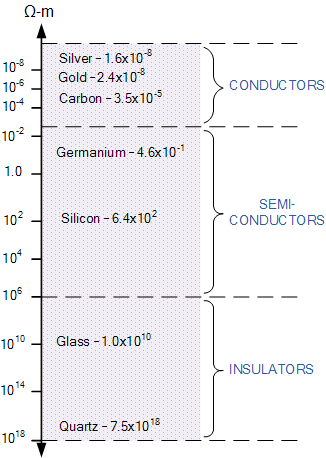
\includegraphics[width=0.3\linewidth]{figs/resistivity.png}
\end{figure}

\subsection{Conductors}
From above we now know that Conductors are materials that have very low values of resistivity, usually in the micro-ohms per metre. This low value allows them to easily pass an electrical current due to there being plenty of free electrons floating about within their basic atom structure. When a positive voltage potential is applied to the material these “free electrons” leave their parent atom and travel together through the material forming an electron drift. In other words a current.

Examples of good conductors are generally metals such as Copper, Aluminium, Silver or non metals such as Carbon because these materials have very few electrons in their outer “Valence Shell”, resulting in them being easily knocked out of the atom’s orbit. This allows them to flow freely through the material until they join up with other atoms, producing a “Domino Effect” through the material thereby creating an electrical current. Copper and Aluminium is the main conductor used in electrical cables as shown.
Generally speaking, most metals are good conductors of electricity, as they have very small resistance values, usually in the region of micro-ohms per metre. While metals such as copper and aluminium are very good conducts of electricity, they still have some resistance to the flow of electrons and consequently do not conduct perfectly.

The energy which is lost in the process of passing an electrical current, appears in the form of heat which is why conductors and especially resistors become hot. Also the resistivity of conductors increases with ambient temperature because metals are also generally good conductors of heat. \cite{diode-basics}.

\subsection{Insulators}
Insulators on the other hand are the exact opposite of conductors. They are made of materials, generally non-metals, that have very few or no “free electrons” floating about within their basic atom structure because the electrons in the outer valence shell are strongly attracted by the positively charged inner nucleus.

So if a potential voltage is applied to the material, no current will flow as there are no electrons to move and which gives these materials their insulating properties.

Insulators also have very high resistances, millions of ohms per metre, and are generally not affected by normal temperature changes (although at very high temperatures wood becomes charcoal and changes from an insulator to a conductor). Examples of good insulators are marble, fused quartz, p.v.c. plastics, rubber etc.

Insulators play a very important role within electrical and electronic circuits, because without them electrical circuits would short together and not work. For example, insulators made of glass or porcelain are used for insulating and supporting overhead transmission cables while epoxy-glass resin materials are used to make printed circuit boards, PCB’s etc. while PVC is used to insulate electrical cables as shown. \cite{diode-basics}.

\subsection{Semiconductors}

Semiconductors materials such as silicon (Si), germanium (Ge) and gallium arsenide (GaAs), have electrical properties somewhere in the middle, between those of a “conductor” and an “insulator”. They are not good conductors nor good insulators (hence their name “semi”-conductors). They have very few “free electrons” because their atoms are closely grouped together in a crystalline pattern called a “crystal lattice”. \cite{diode-basics}.  The outermost electrons of the atoms, the valence electrons, are distributed in a way that defines and holds together the structure of the crystal.

\begin{figure}[H]
\centering
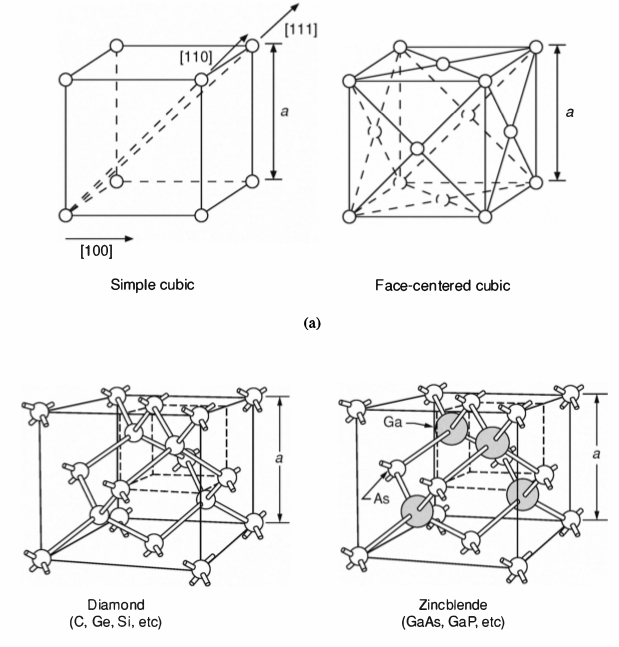
\includegraphics[scale=0.3]{figs/crystal_structure.png}
\caption{Crystal structure of important semiconductors. a) Possibilities of arrangement. b) Arrangement of silicon (Si) and Gallium arsenide (GaAs). Pure silicon crystallizes in a diamond crystal, Gallium arsenide crystallizes in a so called Zincblende structure \cite{book:VLSI}.}
\end{figure}

\subsection{Energy Band Diagrams}
We classify crystals and other solids according to their electrical conductivity into \textbf{insulators}, \textbf{semiconductors}, and \textbf{conductors or metals} in the order of increasing conductivity. Semiconductors are at an intermediate conductivity level, a special property making them suitable for transistors because their conductivity is tunable. It can be modulated by varying the electrical boundary conditions and by introducing atoms of foreign elements into the crystal structure (so called \textbf{impurity doping}).\\
The conductivity of a solid is dependent on the amount of mobile electrons in the solid. Electrons can either be bound to an ion or can be mobile within the solid. Electrical currents are then carried by the motion of the mobile valence electrons. In order to be mobile, the electrons must acquire a minimum energy to break free. The electrons in solids can only be in certain ranges, so called \textbf{energy bands}, and must avoid the forbidden ranges, so called \textbf{energy gaps or band gaps}.

\begin{figure}[H]
\centering
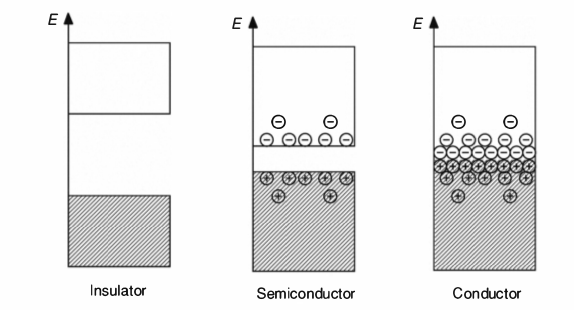
\includegraphics[scale=0.5]{figs/energybands.png}
\caption{The schematic energy bands of an insulator, a semiconductor and a conductor. The hatched areas symbolize the states that are occupied by electrons at zero temperature. At non-zero temperature, some electrons occupy higher energy states leaving ''holes'' in the unoccupied lower-energy states. For insulators, the energy bands are either completely filled or empty, as all electrons are bound. A semiconductor has almost full or almost empty bands and the current can only flow under certain conditions. A conductor has partly filled bands within which electrons can move \cite{book:VLSI}.}
\end{figure}

Valence bands in semiconductors are almost filled, conductance bands almost empty. A concept simplifying the view on semiconductors is that unoccupied states in a valence band are denoted as holes, being positively charged particles.

\begin{figure}[H]
\centering
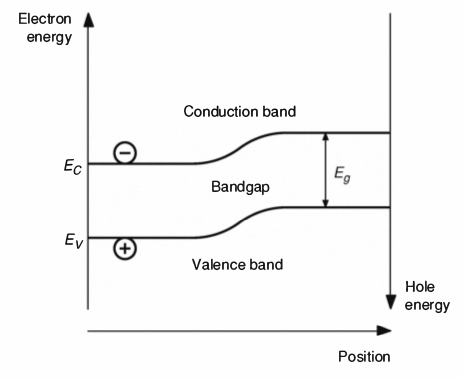
\includegraphics[scale=0.5]{figs/bandgap.png}
\caption{Valence and conduction band of a semiconductor. The energy is plotted as a function of position in one dimension. The energy of the band gap \(E_g\) denotes the difference between the lowest conduction band energy and the highest valence band energy. The band edges tell us the minimum amount of energy an electron has to acquire or lose to bridge the bandgap \cite{book:VLSI}.}
\end{figure}

\subsection{Impurity doping}

The conductivity of a semiconductor is increased significantly by impurity doping. By replacing several atoms of the semiconductor crystal structure by a different element (\textbf{a donor impurity} if it has a valence electron more, \textbf{an acceptor impurity} if it has a valence electron less than the semiconductor atom), we get \textbf{more unbound electrons/holes} as the impurity atom itself is electrically neutral and the electron/hole can move freely.

\begin{figure}[H]
\centering
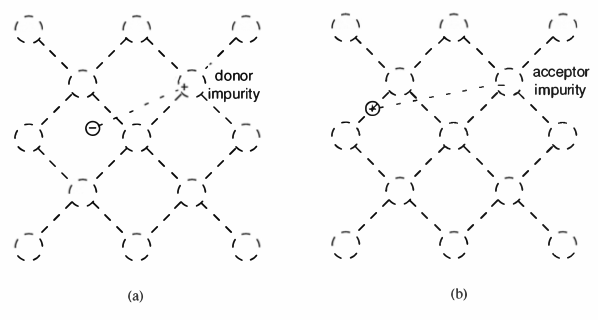
\includegraphics[scale=0.4]{figs/impurity_doping.png}
\caption{Semiconductor with a) donor and b) acceptor impurity doping. The excess charge carrier is only loosely bound to the ion cores (dashed circles) \cite{book:VLSI}.}
\end{figure}

The introduction of donors moves the Fermi level from near the center of the bandgap further towards the conduction-band edge, whereas the
introduction of acceptors moves it closer to the valence-band edge. Higher acceptor doped semiconductors are called \textbf{p-type}, higher donor doped semiconductors are called \textbf{n-type}. Too strongly doped semiconductors have a Fermi level within the valence or conductance band and therefore are similar to metals. Common doping elements are phosphorus (P), arsenic (As) as donors and boron (B) as acceptor.\\
The mobile charge carriers that are dominant in the semiconductor in thermal equilibrium are the majority carriers, the sparser ones are the minority carriers.

\subsubsection{n-type semiconductor}
In N-type semiconductors there are:

\begin{enumerate}
\item The Donors are positively charged.
\item There are a large number of free electrons.
\item A small number of holes in relation to the number of free electrons.
\end{enumerate}

\subsubsection{p-type semiconductor}
\begin{enumerate}
\item The Acceptors are negatively charged.
\item There are a large number of holes.
\item A small number of free electrons in relation to the number of holes.
\end{enumerate}

\subsection{Carrier concentrations at Thermal equilibrium}
Thermal energy makes some electrons move from the lower-energy states to the higher-energy states. The occupancy of energy states is described by the \textbf{Fermi-Dirac distribution} (\(E_F\) denotes the \textbf{Fermi level}, the energy at which the occupation probability is 0.5, k= Boltzmann constant, T=absolute Temperature).

\begin{align*}
F(E) = \frac{1}{1+e^{\frac{E-E_F}{kT}}}
\end{align*}

Typical impurity doping concentration, \(E_F\) is well separated from the valence and conduction band edges (\(|E-E_F| >> kT\)), thus we can use the Boltzmann distribution
\begin{align*}
F(E) = e^{-\frac{E-E_F}{kT}}
\end{align*}
This probability distribution is the reason for the exponential characteristics of diodes and transistors. The fermi level in an undoped semiconductor is usually halfway between the valence and conduction band.

\subsection{Current densities and flows}
By historical definition the electron is assigned the negative elementary charge \(-q\) , where we define \(q\) to be positive. However, the direction of the current density is defined as the direction of positive charge flow.\\ For each carrier type the current flow is due to two basic mechanisms, namely diffusion and drift.
\textbf{Diffusion} is a term borrowed from gas dynamics. It describes the process by which a net particle flow is directed from a region of higher particle density to a region of lower particle density along the density gradient. As we shall see, diffusion determines the current flow in diodes and, within the operating range mainly considered here, in transistors. Diffusion also governs the ion flows in biological neurons.\\
\textbf{Drift} currents are caused by electric fields.

\subsection{p-n Junction Diode}
The fundamental semiconductor device is the p-n junction diode. It is built from an n-type semiconductor and a p-type semiconductor, which, when brought into physical contact, give rise to a net electron flow from n-type to p-type region and a net hole flow from p-type to n-type region. The diffusing minority carriers recombine with majority carriers in the vicinity of the junction and therefore the junction gets depleted of mobile charge carriers, hence its name \textbf{depletion region or space-charge region}. 

\begin{figure}[H]
\centering
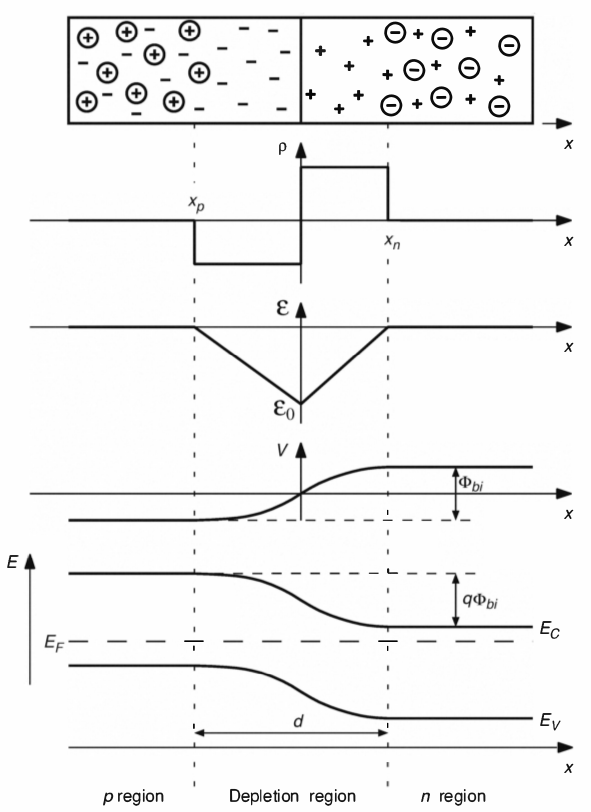
\includegraphics[scale=0.4]{figs/depletion_region.png}
\caption{Characteristics of an abrupt p-n junction in thermal equilibrium with space-charge distribution \(\rho\), electric field distribution \(\mathcal{E}\), potential distribution \(V\). and energy-band diagram \(E\)\cite{book:VLSI}.}
\end{figure}

The depletion region on the n-type side of the junction is depleted of donor electrons and has surplus protons, the p-type side of the junction is depleted of acceptor holes (filled with the donor electrons) and so has surplus electrons. This builds up an electric field pulling the majority carriers back into the other direction. In thermal equilibrium, diffusion and drift currents balance each other out and no net current flow is observed. The offset between the energy bands bordering the depletion region is an electrical potential called \textbf{built-in potential or diffusion potential \(\Phi_{bi}\)}.

\subsection{Forward and Reverse Bias}

In a p-n junction, a net current flow through the diode is generated by applying a potential difference to it. A positive voltage difference applied to the p-type region relative to the n-type region is called a \textbf{forward bias} and the corresponding current is called \textbf{forward current}, a positive voltage difference applied to the n-type region relative to the p-type is called a \textbf{reverse bias}, and the corresponding current \textbf{reverse current}. In a steady state, the total current density must be constant throughout the diode. The electron current in the n-type region is transformed into a hole current in the p-type region. The applied voltage \(V\) appears across the depletion region as a change in the built-in voltage and thus modifies the width of the depletion region.\\
A \textbf{forward bias} shrinks the step across the junction. The positive potential applied to the p-type material repels the holes, while the negative potential applied to the n-type material repels the electrons. With increasing forward-bias voltage, the depletion zone eventually becomes thin enough that the zone's electric field cannot counteract charge carrier motion across the p–n junction, as a consequence reducing electrical resistance. The electrons that cross the p–n junction into the p-type material (or holes that cross into the n-type material) will diffuse in the near-neutral region. The forward current in the p-n junction when it is forward-biased involves electrons from the n-type material moving across the junction and combining with holes in the p-type material. Electrons can then proceed further onward by jumping from hole to hole, so the holes can be said to be moving to the opposite direction in this process.

\begin{figure}[H]
\centering
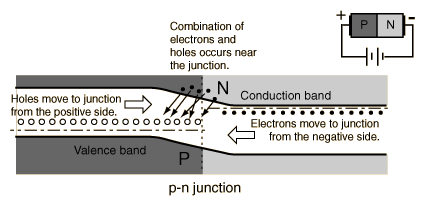
\includegraphics[scale=0.8]{figs/forward_bias.png}
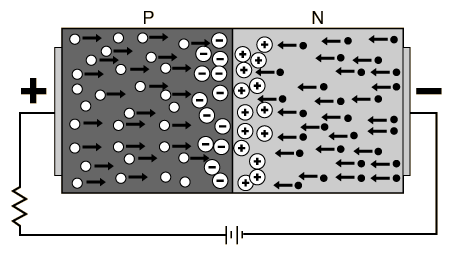
\includegraphics[scale=0.8]{figs/forward_bias2.png}
\caption{Forward biasing of an p-n junction. The white dots (holes) and black dots (electrons) are pushed away and reduce the size of the depletion region.}
\end{figure}

A \textbf{reverse bias} expands the step across the junction. To reverse-bias the p-n junction, the p side is made more negative, making it "uphill" for electrons moving across the junction. This will cause a transient current to flow as both electrons and holes are pulled away from the junction. When the potential formed by the widened depletion layer equals the applied voltage, the current will cease except for the small thermal current.

\begin{figure}[H]
\centering
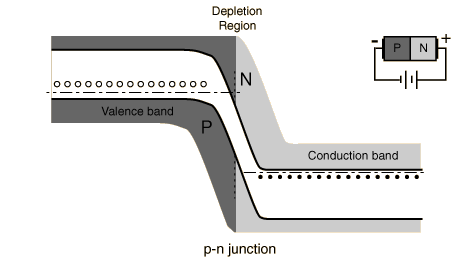
\includegraphics[scale=0.8]{figs/reverse_bias.png}
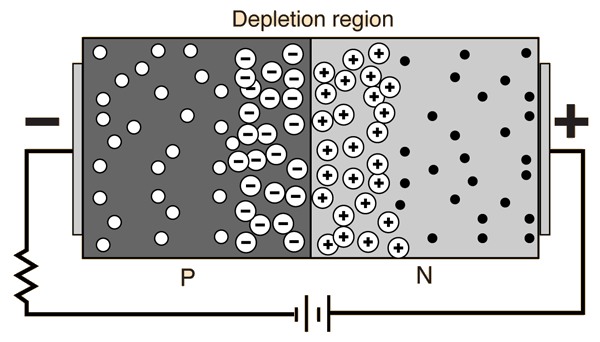
\includegraphics[scale=0.6]{figs/reverse_bias2.png}
\caption{Reverse biasing of an p-n junction.}
\end{figure}

\begin{figure}[H]
\centering
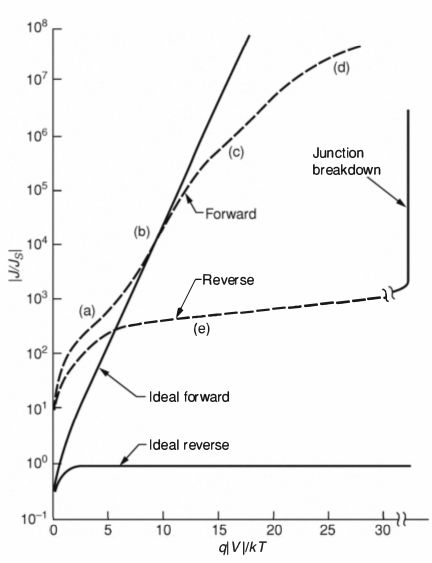
\includegraphics[scale=0.5]{figs/biasing.png}
\caption{Biasing of an p-n junction \cite{book:VLSI}.}
\end{figure}

For large reverse biases, a phenomenon called \textbf{junction breakdown} occurs that expresses itself in a sudden increase of reverse current at a certain reverse voltage. For silicon with typical impurity doping concentrations this effect is due to impact ionization: The generation of electron-hole pairs by collision with an electron or hole that has acquired sufficient kinetic energy in the electric field of the depletion region. A charge carrier may create multiple electron-hole pairs during its transition through the depletion region. The generated carriers can in turn create electron-hole pairs if they acquire sufficient energy, and so on. This effect is known as avalanche multiplication.

%Ben End

\subsection{MIS and MOS structure}

\subsubsection{MIS}  Metal-Insulator-Semiconductor, consists of a conductor and a semiconductor, separated by thin insulation layer.
\subsubsection{MOS}  Metal-Oxide-Silicon, a version of MIS, in which silicon dioxide ($SiO_2$) is used as oxide.

The traditional metal–oxide–semiconductor (MOS) structure is obtained by growing a layer of silicon dioxide ($SiO_2$) on top of a silicon substrate and depositing a layer of metal or polycrystalline silicon (the latter is commonly used). As the silicon dioxide is a dielectric material, its structure is equivalent to a planar capacitor, with one of the electrodes replaced by a semiconductor.

When a voltage is applied across a MOS structure, it modifies the distribution of charges in the semiconductor. If we consider a p-type semiconductor (with $N_A$ the density of acceptors, p the density of holes; p = $N_A$ in neutral bulk), a positive voltage, $V_{gb}$, from gate to body (see figure \ref{fig:MOS_Structure}) creates a depletion layer by forcing the positively charged holes away from the gate-insulator/semiconductor interface, leaving exposed a carrier-free region of immobile, negatively charged acceptor ions.
\begin{figure}[H]
\centering
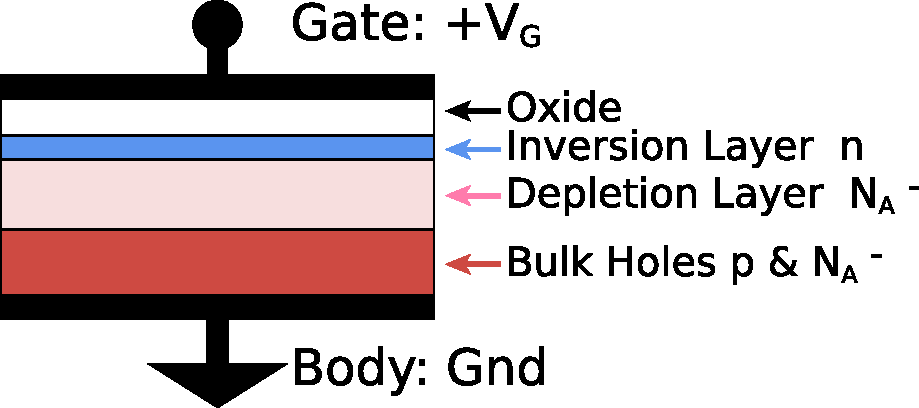
\includegraphics[width=0.6\linewidth]{figs/MOS_Capacitor.pdf}
\caption{Metal–oxide–semiconductor structure on p-type silicon.}
\label{fig:MOS_Structure}
\end{figure}
 If $V_{gb}$ is high enough, a high concentration of negative charge carriers forms in an inversion layer located in a thin layer next to the interface between the semiconductor and the insulator. Unlike the MOSFET, where the inversion layer electrons are supplied rapidly from the source/drain electrodes, in the MOS capacitor they are produced much more slowly by thermal generation through carrier generation and recombination centers in the depletion region. Conventionally, the gate voltage at which the volume density of electrons in the inversion layer is the same as the volume density of holes in the body is called the threshold voltage. When the voltage between transistor gate and source ($V_{gs}$) exceeds the threshold voltage ($V_{th}$), it is known as overdrive voltage.

This structure with p-type body is the basis of the n-type MOSFET, which requires the addition of an n-type source and drain regions \cite{wiki:MOSFET}.

%Joachim Start
\subsection{MOS Transistor Structure}

\subsubsection{CMOS}  Complementary Metal Oxide Silicon, a MOS process in which both nFET and pFET are fabricated on the same substrate.
\subsubsection{MOSFET} Metal-Oxide-Semiconductor Field-Effect Transistor, built using MOS and a p-n junction diode.

The metal–oxide–semiconductor field-effect transistor (MOSFET, MOS-FET, or MOS FET) is a type of transistor used for amplifying or switching electronic signals.
In neuromorphic engineering, we use the MOSFET in the subthreshold domain because the current here is exponentially dependent on the control voltages of the MOSFET just as the ionic conductances of a neuron are exponentially dependent on its membrane potential. Furthermore when MOSFETs are operated in the subthreshold domain, they draw small currents so power consumption is reduced.

\begin{figure}[H]
  \centering

  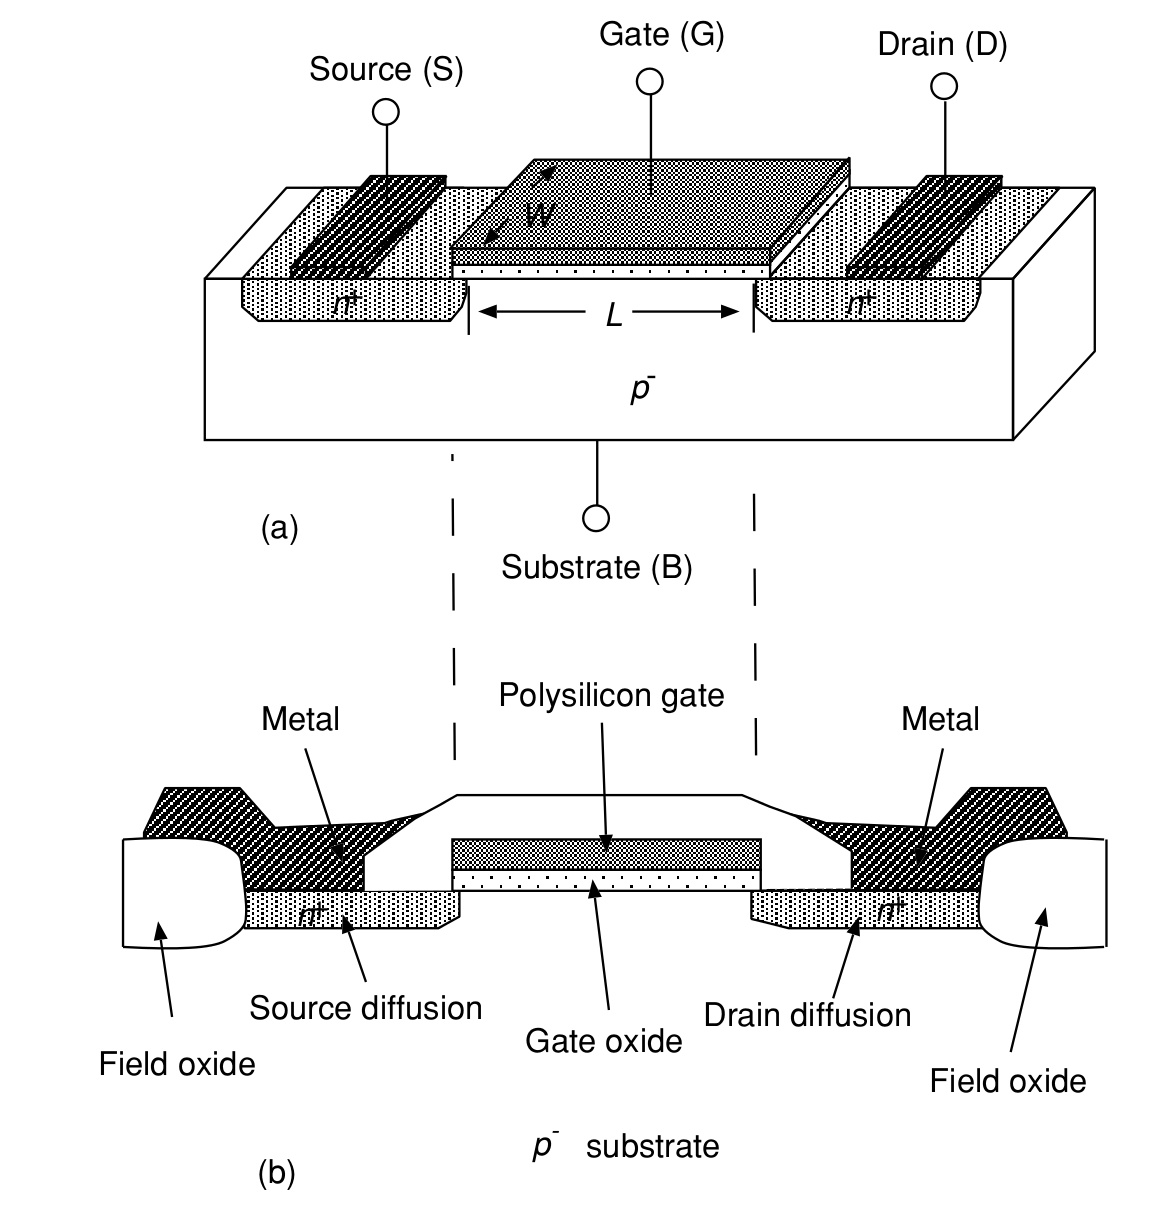
\includegraphics[scale=0.8]{figs/MOSFET_Structure.jpg}
  \caption{Structure of an n-type MOSFET in a p-body. The MOSFET has four terminals; the drain (D), the source (S), the gate (G), and the bulk (B). (a) Pictorial view of the MOSFET. (b) A more realistic picture of a cross-section of a fabricated MOSFET. Note that the gate oxide is much thinner than the field oxide. \cite{book:VLSI}}
  \label{fig:MOSFET_Structure}
\end{figure}\bigskip

\subsection{MOS Transistor Types}
\subsubsection{n-type}
    Because the n+ source and drain regions can supply a lot of electrons to the channel, this device is called an n-channel MOSFET (nFET,n-type MOSFET, NMOS) \cite{book:VLSI}
\subsubsection{p-type}
   In p-channel MOSFET (pFET,p-type MOSFET, PMOS) , the charge in the channel is carried by holes supplied from the source and drain regions.
    
\bigskip\subsection{MOS Transistor in Substrate}
Most CMOS processes use a p-type starting substrate.  The nFETs rest in the common $p^-$ substrate, and the pFETs rest in
n-wells within the substrate as shown in Fig. \ref{fig:MOSFET_Physical_Structure}

\begin{figure}[H]
  \centering
  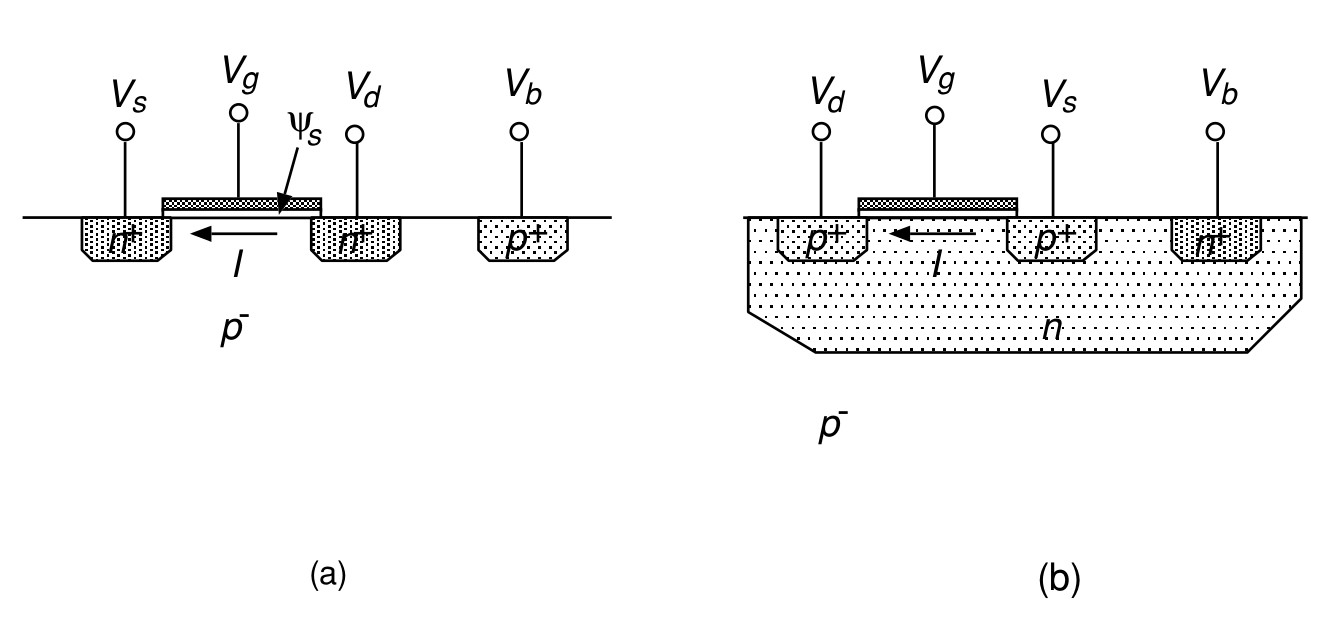
\includegraphics[scale=0.8]{figs/MOSFET_Physical_structure.jpg}
  \caption{Physical structure of (a) an nFET and (b) a pFET in a common $p^-$ substrate. The pFET rests in a n-well within the substrate. \cite{book:VLSI}}
  \label{fig:MOSFET_Physical_Structure}
\end{figure}

\subsection{Transistor biasing}
For a transistor to work properly, we need certain bias conditions.
These bias conditions guarantee that there will only be a small reverse leakage current at these junctions and that most of the transistor’s current will flow in the channel.
\subsubsection{nFET biasing}
To ensure only a small leakage current between the $n^+$ regions to the p-substrate, the junctions have to be reverse biased.
To do this, the drain voltage $V_d$ and the source voltage $V_s$ of the nFET should be greater than or equal to the bulk voltage $V_b$:
\[V_{sb}=V_s-V_b \geq 0\]
\[V_{db}=V_d-V_b \geq 0\]


The $n^+$ region biased at the higher voltage is called the drain, and the other $n^+$ region is called the source. Because electrons are negatively charged, the direction of positive current flow $I$ is from drain to source, even though the carriers flow from source to drain. The bulk of the nFET is tied to the lowest voltage ( $V_{ss}$ ). \cite{book:VLSI}

\subsubsection{pFET biasing}
In pFET , the $p^+$ regions should be biased negative relative to the bulk to reverse-bias the pn junctions.
\[V_{sb} \leq 0\]
\[V_{db} \leq 0\]
The n-type bulk (or n-well) of the pFET should be biased higher (usually $V_{dd}$.  In a $p^-$ substrate, where the pFET rests in an n-well, the well is connected to $V_{dd}$, and the substrate to $V_{ss}$.) For a pFET, the $p^+$ region which is biased at the higher voltage is called the source and the other $p^+$ region is called the drain.


\subsection{MOS Transistor Channel}
The region underneath the gate and between the source and drain regions is called the channel. The channel has a width W, and a length L. The channel is insulated from the gate above by a layer of silicon dioxide. The gate is made of heavily doped (low resistivity) polycrystalline silicon.
\cite{book:VLSI}

\subsection{MIS Operation Domains}
In a typical MIS structure, the insulator layer is sufficiently thick that it cannot be crossed by charge carriers under normal operating conditions and sufficiently thin that the charge on the conductor can influence the charge distribution in the semiconductor via the electrostatic potential it induces. A positive
charge on the conductor attracts mobile electrons from the semiconductor to
the semiconductor-insulator interface and repels mobile holes away from the
interface. Conversely, a negative charge on the conductor attracts holes and
repels electrons.\\
\textbf{Important: }Relevant here is the type of substrate (p or n) the channel is made of, which is p in nFET and n in pFET!
\begin{figure}[H]
  \centering
  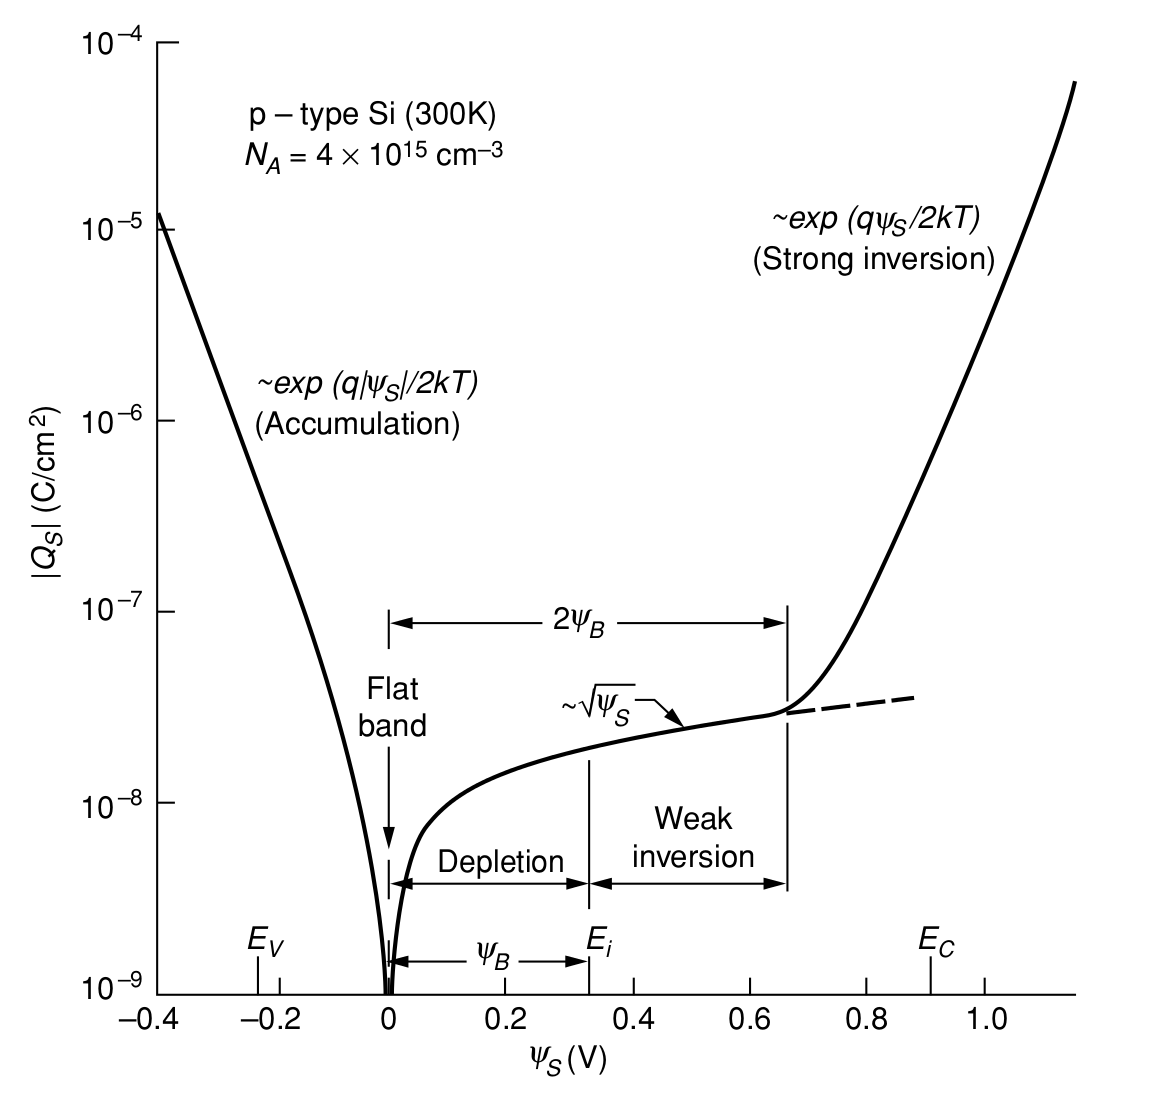
\includegraphics[scale=1]{figs/operation_domains.png}
  \caption{Dependence of the area charge $Q_s$ on the surface potential for p-type silicon with acceptor density $N_A = 4 \times \unit[10^{15}]{cm^{-3}}$ at room temperature. The same effects are observed in n-type semiconductors, if the sign of the charge on the conductor is reversed \cite{book:VLSI}.}
  \label{fig:coperation_domains}
\end{figure}

\begin{figure}[H]
\centering
  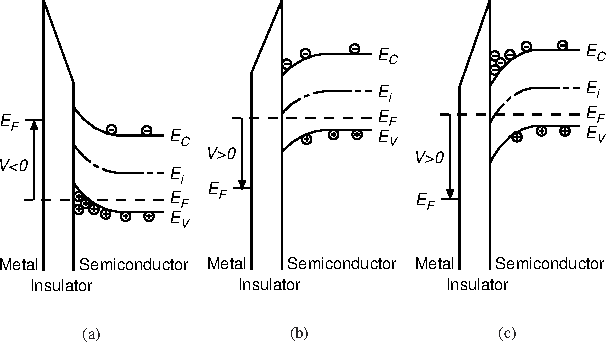
\includegraphics[scale=1]{figs/operation_domains2.pdf}
  \caption{Energy-band diagrams of an ideal MIS diode with applied bias for a p-type semiconductor in (a) accumulation, (b) depletion, and (c) inversion \cite{book:VLSI}.}
\end{figure}

\subsubsection{Accumulated Transistor Channel}
Accumulation happens when a charge on the gate attracts a lot of majority carriers on the surface of the semiconductor underneath it.\\
For a p-substrate channel (default), as shown in figure \ref{fig:channel_accumulated}, a negative voltage on the gate means mobile electrons on the gate. These electrons (negatively charged) attract positive charges on the semiconductor surface underneath it, leading to accumulation of them. Since positive charges (holes) are the majority carrier in p-substrate, we call this situation accumulation.\\\\
In a n-substrate channel, positive charge on the gate leads to accumulation of electrons (majority carriers in n-substrate) on the channel surface.
\begin{figure}[H]
  \centering
  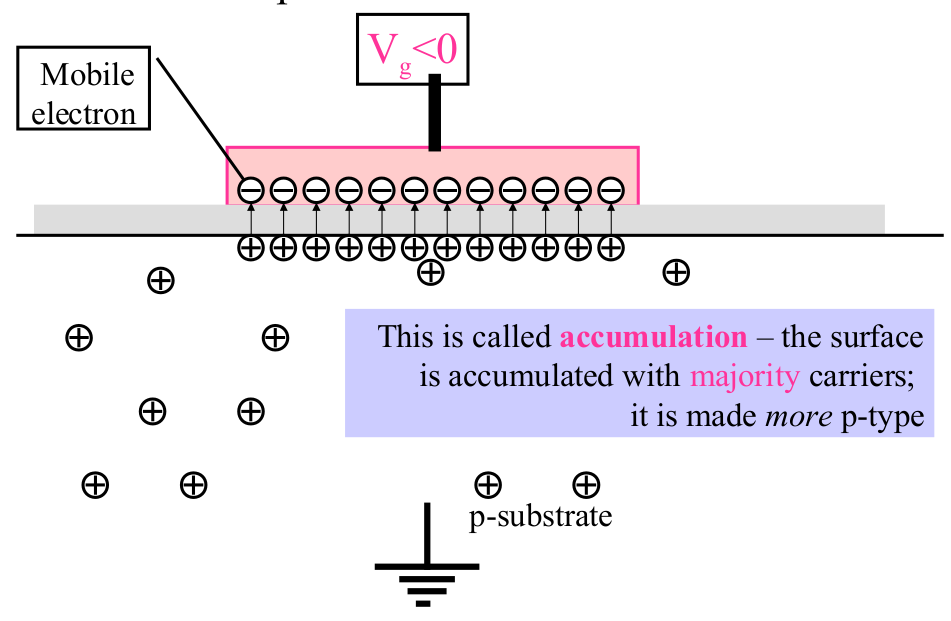
\includegraphics[scale=1]{figs/channel_accumulation.png}
  \caption{Accumulated Transistor Channel \cite{lec2}}
  \label{fig:channel_accumulated}
\end{figure}


\subsubsection{Flat-Band Transistor Channel}
In an ideal MIS diode, with no bias applied, the work function of the metal and the semiconductor are the same.  The Fermi levels line up and the energy bands in the semiconductor are flat. $\rightarrow$ Flat-Band Condition \cite{book:VLSI}\\
With $V_g=V_{fb}=0$, the majority carrier density is constant and equal to the dopant density.
\begin{figure}[H]
  \centering
  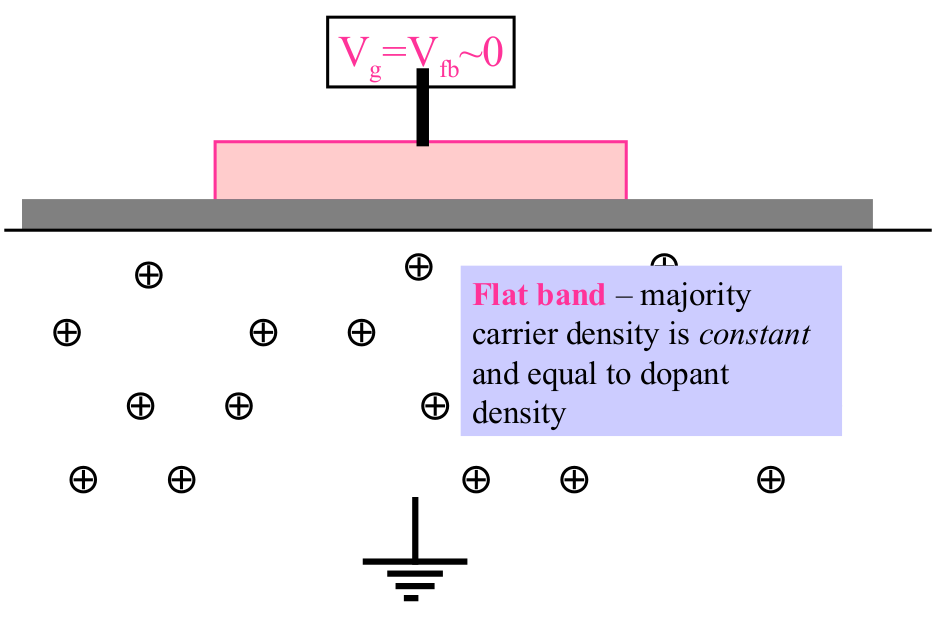
\includegraphics[scale=1]{figs/channel_flat_band.png}
  \caption{Flat-Band Transistor Channel \cite{lec2}}
  \label{fig:channel_flat_band}
\end{figure}

\subsubsection{Depleted Transistor Channel}

For a p-substrate channel, if we put a positive subthreshold voltage on the gate (positive charges), we repulse positive majority carriers on the semiconductor surface. $\rightarrow$ Depletion of majority carriers.\\
For a n-substrate channel, the same happens if we put a subthreshold negative charge on the gate. $\rightarrow$ Depletion of electrons (majority carrier in n substrate) on the semiconductor surface.

\begin{figure}[H]
  \centering
  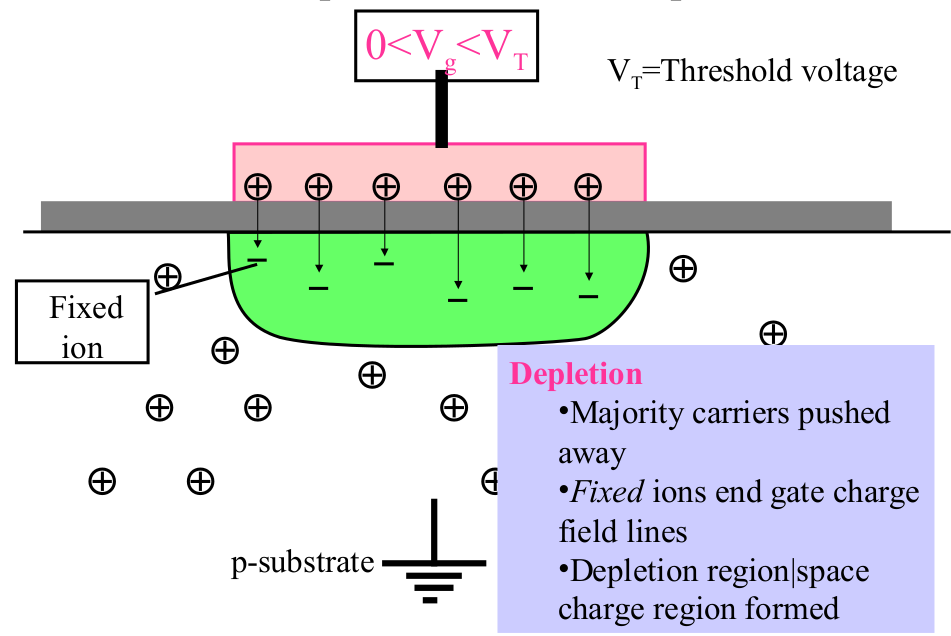
\includegraphics[scale=1]{figs/channel_depletion.png}
  \caption{Depleted Transistor Channel \cite{lec2}}
  \label{fig:channel_depletion}
\end{figure}

\subsubsection{Inverted Transistor Channel}
For a depleted p-substrate channel, if we now further increase the positive charge on the gate, we will reach a point where we start attracting negative minority carriers on the semiconductor surface. The surface becomes inverted. (p-type $\rightarrow$ n-type and vice versa in n substrate)  $\rightarrow$ Inversion
\begin{figure}[H]
  \centering
  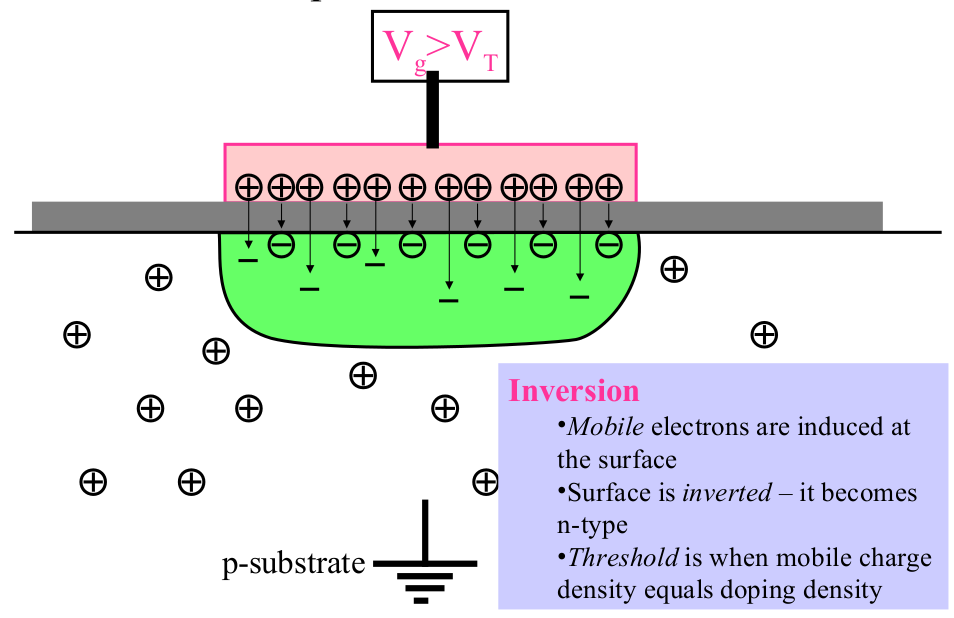
\includegraphics[scale=1]{figs/channel_inversion.png}
  \caption{Inverted Transistor Channel \cite{lec2}}
  \label{fig:channel_inversion}
\end{figure}
%Joachim End
%Ben Start
\subsubsection{Strongly Inverted Transistor Channel}
The minimum voltage that has to be applied to the MIS structure to obtain
strong inversion is called threshold voltage.

%Ben End

\subsection{Readings}
\begin{enumerate}
\item AVLSI p. 28-45
\end{enumerate}

\todo[inline]{Add more basic theory (e.g. definition and meaning of $U_T$)}
\end{document}